\documentclass[12pt,letterpaper]{article}

% Gabarit officiel INF8770 : police, marges et interligne conservés.
\usepackage[utf8]{inputenc}
\usepackage[T1]{fontenc}
\usepackage[french]{babel}
\usepackage{newtxtext,newtxmath}
\usepackage[margin=2cm]{geometry}
\usepackage{graphicx}
\usepackage{booktabs}
\usepackage{amsmath}
\usepackage{listings}
\usepackage{xcolor}
\usepackage{hyperref}
\usepackage{caption}
\usepackage{microtype}
\usepackage{float}

\hypersetup{colorlinks=true,linkcolor=black,citecolor=blue!70!black,urlcolor=blue!80!black}
\definecolor{codegreen}{rgb}{0,0.6,0}
\definecolor{codegray}{rgb}{0.5,0.5,0.5}
\definecolor{codepurple}{rgb}{0.58,0,0.82}
\definecolor{backcolour}{rgb}{0.97,0.97,0.97}
\lstdefinestyle{mystyle}{
    backgroundcolor=\color{backcolour}, commentstyle=\color{codegreen},
    keywordstyle=\color{blue}\bfseries, numberstyle=\tiny\color{codegray},
    stringstyle=\color{codepurple}, basicstyle=\ttfamily\footnotesize,
    breaklines=true, captionpos=b, keepspaces=true, numbers=left,
    numbersep=7pt, showspaces=false, showstringspaces=false, showtabs=false,
    tabsize=4, frame=single, rulecolor=\color{black!20}}
\lstset{style=mystyle}

\begin{document}
\pagenumbering{roman}
\begin{titlepage}
    \centering
    \vspace*{0.5cm}
    
\includegraphics[width=0.45\textwidth]{logo_polytechnique.png}\\[1.5cm]
    {\Huge \textbf{INF8770 : Technologies Multimédias}}\\[0.5cm]
    {\LARGE \textbf{TP1 : Compression sans perte de textes}}\\[0.3cm]
    {\Large Automne 2026}\\[2cm]
    {\large \textbf{Équipe :}}\\[0.3cm]
    {\normalsize Benjamin Dupuis \quad (Matricule : 2557585)}\\[0.15cm]
    {\normalsize Gaël Lienard \quad (Matricule : 2489319)}\\[1.5cm]
    {\large \textbf{Chargé de travaux pratiques :}}\\[0.3cm]
    {\normalsize Mohamed Aziz Younes}\\[2cm]
    \vfill
    {\normalsize Département de génie informatique et génie logiciel}\\
    {\normalsize Polytechnique Montréal}\\[0.5cm]
    {\small Date de remise : 28 septembre 2026}
    \thispagestyle{empty}
\end{titlepage}

\newpage
\pagenumbering{arabic}
\setcounter{page}{1}
\tableofcontents
\newpage

\section{Introduction}
Nous comparons Huffman à deux méthodes sur trois fichiers : un programme Python, un texte littéraire et un fichier météo au format CSV. Le but est de réduire leur taille sans perdre d'information, puis de vérifier que le décodage restitue les fichiers d'origine.

\section{Analyse exploratoire}
\subsection{Question 1 : structure des fichiers}
Les fréquences des octets sont inégales : l'entropie mesurée va de 4,368 à 4,969 bits par octet, contre 8 bits pour un octet non compressé. Huffman peut donc réduire la taille en donnant des codes courts aux octets fréquents. En revanche, il ne tient pas compte directement des suites de caractères qui se répètent.

Le code contient des espaces, des mots-clés et des structures récurrentes. Le CSV répète ses en-têtes et certains champs. Le texte contient des mots récurrents, mais peu de longues suites identiques. Ces différences expliquent pourquoi une méthode peut bien fonctionner sur un fichier et moins bien sur un autre.

\begin{table}[H]
    \centering
    \caption{Caractéristiques mesurées des fichiers, en octets, bits/octet et octets par plage.}
    \label{tab:analyse}
    \small
    \begin{tabular}{lrrrr}
        \toprule
        Fichier & Taille [octets] & $H_0$ [bits/octet] & Plage moyenne [octets] & Plage max. [octets] \\
        \midrule
        Code Python & 3\,844 & 4,368 & 1,33 & 78 \\
        Littéraire français & 5\,092 & 4,422 & 1,02 & 2 \\
        Météo CSV & 26\,515 & 4,969 & 1,06 & 3 \\
        \bottomrule
    \end{tabular}
\end{table}

L'entropie est calculée par $H_0=-\sum_b p_b\log_2p_b$. Les plages de même octet sont courtes dans le texte et le CSV. Une compression par plages (RLE) est donc peu adaptée à ces deux fichiers.

\subsection{Question 2 : méthodes testées}
Nous avons d'abord essayé une prédiction différentielle suivie du codage de Golomb, une méthode étudiée en cours~\cite{cours}. La prédiction transforme chaque octet en différence avec le précédent; le codage ZigZag rend les différences négatives non négatives. Cette méthode ne donne pas de meilleurs résultats que Huffman dans nos essais.

Nous avons ensuite retenu LZ77. Cette méthode remplace une suite déjà rencontrée par une référence, ce qui devrait aider pour le code et les champs répétés du CSV. Le texte littéraire contient moins de longues répétitions exactes; le coût des références risque donc d'y annuler le gain. Les résultats permettent de vérifier cette hypothèse.

\section{Implémentation et évaluation}
\subsection{Question 3 : implémentation}
Le notebook contient Huffman, Golomb prédictif et LZ77, ainsi que leurs essais de décodage. Le code Huffman suit l'exemple vu en cours. Pour LZ77, la fenêtre de recherche fait 32\,768 octets et la longueur maximale examinée est de 258 octets. Une suite répétée de trois octets ou plus devient une référence; sinon, l'octet est écrit tel quel. Le flux LZ77 est empaqueté en octets et inclut le nombre de jetons. Les tests du notebook vérifient la reconstruction des trois fichiers. Les outils utilisés sont Python, NumPy, Matplotlib et AnyTree~\cite{outils}.

La Figure~\ref{fig:residus} montre les résidus de la prédiction ZigZag. Le CSV a les résidus les plus faibles en moyenne, mais cela ne suffit pas à rendre le codage de Golomb plus efficace que Huffman.

\begin{figure}[H]
    \centering
    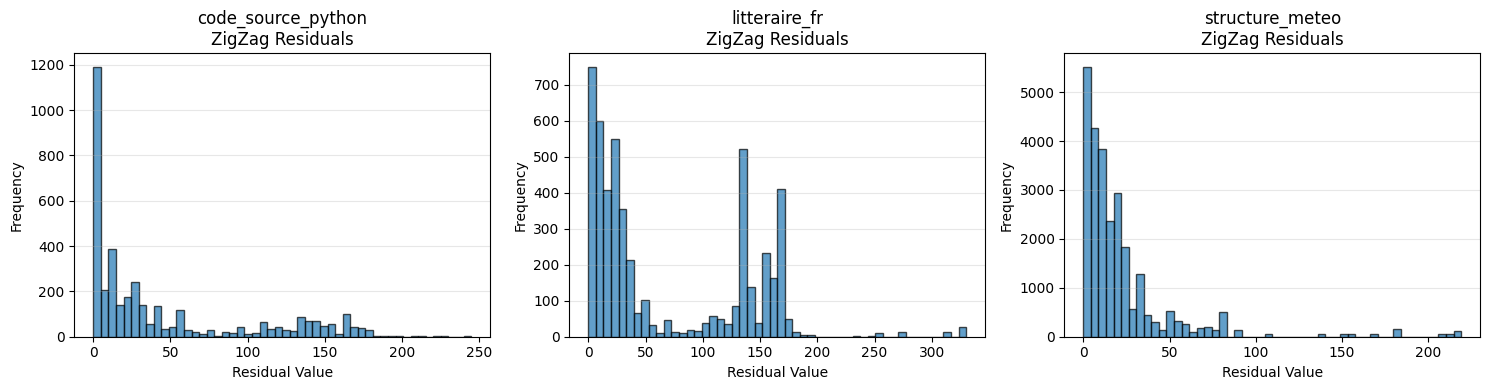
\includegraphics[width=\textwidth]{residus_zigzag.png}
    \caption{Résidus ZigZag après prédiction. Axe horizontal : valeur du résidu [sans unité]. Axe vertical : nombre d'octets [occurrences].}
    \label{fig:residus}
\end{figure}

\subsection{Question 4 : résultats}
Le Tableau~\ref{tab:resultats} reprend les tailles affichées par le notebook. La taille de Huffman comprend une estimation du dictionnaire. La taille de Golomb correspond au nombre de bits divisé par huit; l'en-tête et le remplissage final ne sont pas comptés. Pour LZ77, le flux empaqueté et les quatre octets indiquant le nombre de jetons sont comptés. Les tailles ne comprennent donc pas toutes les mêmes frais de formatage et restent des estimations de cette implémentation.

\begin{table}[H]
    \centering
    \caption{Tailles estimées par le notebook [octets] et pourcentage de la taille originale [\%].}
    \label{tab:resultats}
    \small
    \resizebox{\textwidth}{!}{%
    \begin{tabular}{lrrrr}
        \toprule
        Fichier & Original [octets] & Huffman [octets, \%] & Golomb prédictif [octets, \%] & LZ77 [octets, \%] \\
        \midrule
        Code Python & 3\,844 & 2\,383 (62,0) & 3\,280 (85,3) & 1\,743 (45,3) \\
        Texte français & 5\,092 & 3\,078 (60,4) & 4\,834 (94,9) & 3\,995 (78,5) \\
        Météo CSV & 26\,515 & 16\,761 (63,2) & 19\,830 (74,8) & 7\,420 (28,0) \\
        \bottomrule
    \end{tabular}}
\end{table}

\begin{figure}[H]
    \centering
    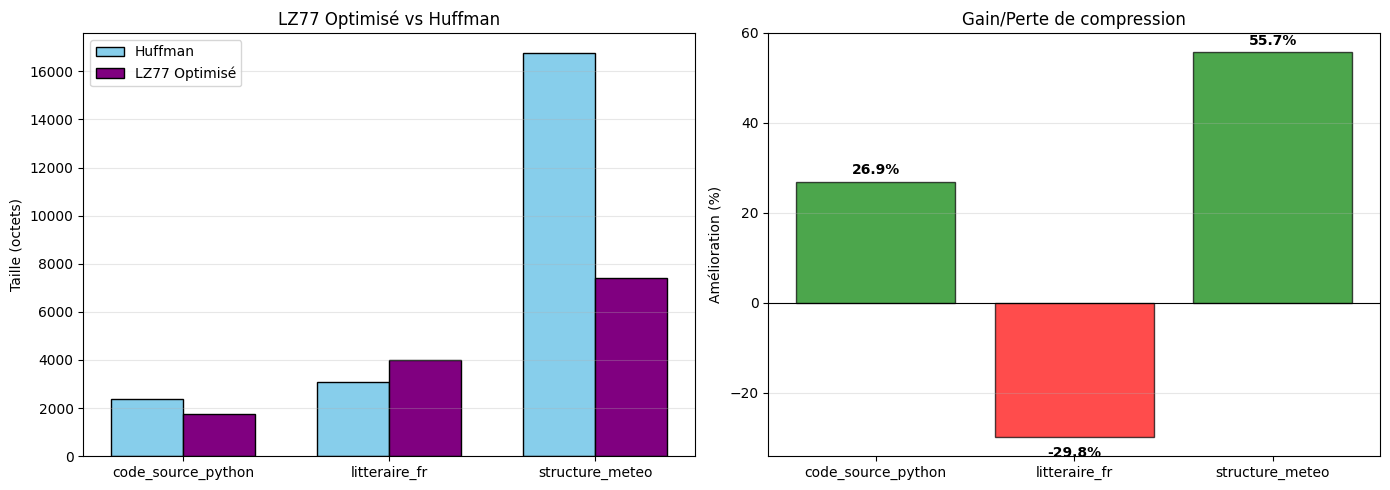
\includegraphics[width=0.88\textwidth]{comparaison_tailles.png}
    \caption{Comparaison Huffman--LZ77 et gain ou perte observé. Les tailles sont en octets; l'amélioration est en pourcentage par rapport à Huffman.}
    \label{fig:tailles}
\end{figure}

LZ77 améliore la taille par rapport à Huffman de 26,9\,\% pour le code et de 55,7\,\% pour le CSV. Pour le texte, il produit un fichier 29,8\,\% plus grand. Les références LZ77 sont efficaces quand les suites répétées sont assez longues; sur le texte, elles coûtent plus cher que les répétitions ne rapportent. Golomb prédictif reste derrière Huffman sur les trois fichiers, et l'ajout d'un deuxième Huffman ne l'améliore pas. Ainsi, le résultat attendu est obtenu pour deux fichiers sur trois, mais pas pour le texte littéraire.

\section{Conclusion}
LZ77 compresse mieux que Huffman pour le code et le CSV, mais moins bien pour le texte littéraire. La méthode n'atteint donc pas l'objectif de surpasser Huffman sur les trois fichiers. Les résultats confirment toutefois que le choix de l'algorithme doit tenir compte des répétitions propres à chaque type de texte.

\begin{thebibliography}{9}
    \bibitem{cours}
    G.-A. Bilodeau, \textit{INF8770, chapitre 2 : compression sans perte}, notes et notebooks du cours.
    \bibitem{outils}
    Documentations de NumPy, Matplotlib et AnyTree : \url{https://numpy.org/doc/}, \url{https://matplotlib.org/stable/} et \url{https://anytree.readthedocs.io/}.
\end{thebibliography}

\end{document}
